%%%%%%%%%%%%%%%%%%%%%%%%%%%
% Práctica 1: Accesibilidad Web
% @uthora: Ana del Carmen Santana Ojeda
% @uthor: Alejandro David Arzola Saavedra
% @date: 25/09/2023
%%%%%%%%%%%%%%%%%%%%%%%%%%%
% Estructura basica de la pagina
\documentclass[a4paper]{article}
\usepackage[utf8]{inputenc}
\usepackage[spanish]{babel}
\usepackage{fancyhdr} %Definimos el estilo de página

% Paquetes adicionales
\usepackage{graphicx,efbox}
\usepackage[headsep=0.2cm]{geometry}
\usepackage[most]{tcolorbox}
\newcommand{\MYhref}[3][black]{\href{#2}{\color{#1}{#3}}}
\usepackage[hyperindex=true, colorlinks=true, linkcolor=black, breaklinks=true, urlcolor=black, citecolor=black, anchorcolor= black]{hyperref}


% Agrega el paquete para personalizar el índice
\usepackage{tocloft}

% Personaliza la apariencia de la entrada "Bibliografía" en el índice
\renewcommand{\cftsecleader}{\cftdotfill{\cftdotsep}}
\renewcommand{\cftsecafterpnum}{\vspace{0.5\baselineskip}}



% Variable de entorno de fecha
\newcommand{\dateToday}{25 de septiembre de 2023}

% Variable de imagenes
\newcommand{\logoULPGC}{ulpgc.png}
\newcommand{\imagenUnicef}{unicef.png}
\newcommand{\imagenTelegram}{telegram.jpeg}
\newcommand{\imagenPortada}{discapacidad_principal.png}
\newcommand{\paginaUnicef}{paginaUnicef.png}
\newcommand{\responsiveUnicef}{responsiveUnicef.png}
\newcommand{\accesibilidadUnicef}{accesibilidadUnicef.png}
\newcommand{\erroresUnicef}{errorUnicef.png}
\newcommand{\aplicacionTelegram}{fotoTelegramMovil.png}
\newcommand{\letraTelegram}{letraTelegram.jpg}
\newcommand{\coloresTelegram}{colores_telegram.jpg}
\newcommand{\idiomaTelegram}{idiomaTelegram.jpg}
\newcommand{\asegurarTelegram}{asegurarTelegram.jpg}
\newcommand{\deshacerTelegram}{deshacerTelegram.jpg}
\newcommand{\numeroTelefono}{numeroTelefonoTelegram.jpg}
\newcommand{\mensajeTelefono}{mensajeTelefonoTelegram.jpg}

%Cambio indice
\addto\captionsspanish{\renewcommand{\contentsname}{Índice}}

\setlength{\headheight}{ 40.2pt}
\pagestyle{fancy}
\lhead{\includegraphics[width=5cm]{\logoULPGC}}\rhead{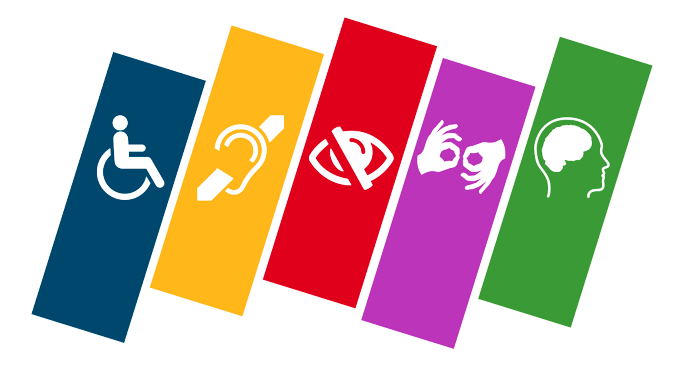
\includegraphics[height=1cm]{discapacidad_principal.png}}

\geometry{a4paper, total={170mm,257mm}, left=35mm, top=20mm, right=35mm}

\begin{document}
    %%%%%%%%%%%%%%%%%%%%%%%%%%%%%%%%%
    %%   Portada del documento
    %%%%%%%%%%%%%%%%%%%%%%%%%%%%%%%%%
    \begin{titlepage}
        \centering
        \vspace*{2cm}
        \includegraphics[width=0.6\textwidth]{\logoULPGC}\par\vspace{1cm}
    
        {\scshape\textbf{\LARGE Práctica 1}}\par
        \vspace{0.6cm}
        {\bfseries}{\Huge Accesibilidad Web}
        \vspace{2cm}
    
        \includegraphics[width = \textwidth, height = 10cm, keepaspectratio]{\imagenPortada}\vspace{1cm}
            
        \begin{tcolorbox}[colback=red!5!white,colframe=white!50!black]
            \centering \Large Programación de Aplicaciones Móviles Nativas \par
            \dateToday
        \end{tcolorbox}

        \vspace{1cm}        
        \begin{tcolorbox}[colback=green!5!white,colframe=green!75!black]
            Autores:
            \tcblower
            Ana del Carmen Santana Ojeda (ana.santana152@alu.ulpgc.es)\par \vspace{0.5cm}
            Alejandro David Arzola Saavedra (alejandro.arzola101@alu.ulpgc.es)
        \end{tcolorbox}
    \end{titlepage}
    
    \newpage
        
    %%%%%%%%%%%%%%%%%%%%%%%%%%%%%%%%%
    % Tabla de contenido de la pagina
    %%%%%%%%%%%%%%%%%%%%%%%%%%%%%%%%%
    \tableofcontents 
    
    \newpage

    %%%%%%%%%%%%%%%%%%%%%%%%%%%
    % Introduccion de la pagina
    %%%%%%%%%%%%%%%%%%%%%%%%%%%
    \section{Introducción}
    \label{sec:introduccion_desarrollo}
    En el contexto de la evaluación de accesibilidad web, se llevará a cabo un análisis exhaustivo del sitio web oficial y una aplicación móvil, en nuestro caso será \textbf{UNICEF}(\textit{United Nations Children's Fund}) y \textbf{Telegram}, como se puede ver en la \textbf{\hyperref[fig:imagen-unicef]{Imagen 1}} e \textbf{\hyperref[fig:imagen-telegram]{Imagen 2}}.\vspace{0.1cm}

    \begin{center}
        \efboxsetup{linecolor=black,linewidth=0.5pt}
        \efbox{\includegraphics[width=0.8\textwidth, height=10cm, keepaspectratio]{\imagenUnicef}}\vspace{0.2cm}\par
        \textbf{Imagen 1: UNICEF\label{fig:imagen-unicef}}
    \end{center}\vspace{0.1cm}

    La accesibilidad web desempeña un papel fundamental en la garantía de que la información y los servicios en línea sean accesibles para todos, independientemente de sus capacidades y discapacidades. \vspace{0.5cm}

    El objetivo de esta evaluación es medir el grado de conformidad de la página web y de la aplicación con las pautas y estándares de accesibilidad web establecidos por el \textit{World Wide Web Consortium (\textbf{W3C})}.\vspace{0.1cm}

    \begin{center}
        \efboxsetup{linecolor=black,linewidth=0.5pt}
        \efbox{\includegraphics[width=0.8\textwidth, height=10cm, keepaspectratio]{\imagenTelegram}}\vspace{0.2cm}\par
        \textbf{Imagen 2: Telegram\label{fig:imagen-telegram}}
    \end{center}\vspace{0.1cm}

    Este análisis se centrará en evaluar diversos aspectos de accesibilidad web, incluyendo la utilización de atributos \textbf{ARIA}(\textit{Accessible Rich Internet Applications}), el uso de textos alternativos para imágenes, la estructura del sitio, el contraste de color, la presencia de contenido sin texto en imágenes y otros aspectos relevantes para garantizar que sea lo más inclusivo y accesible posible.\vspace{0.5cm}

    A continuación, se presentará un resumen detallado de los puntos positivos y negativos encontrados durante la evaluación, junto con recomendaciones para mejorar la accesibilidad web del sitio de \textbf{UNICEF} y \textbf{Telegram}.
            
    \newpage

    %%%%%%%%%%%%%%%%%%%%%%%%%%%
    % Desarrollo de la pagina
    %%%%%%%%%%%%%%%%%%%%%%%%%%%
    \section{Desarrollo\texorpdfstring{\vspace{0.2cm}}{}} 

    \label{sec:desarrollo}
    
    Como hemos comentado anteriormente, hemos seleccionado el sitio web oficial de \textbf{UNICEF}(Fondo de las Naciones Unidas para la Infancia) como podemos ver en la \textbf{\hyperref[fig:imagen-captura-unicef]{Imagen 3}} como objeto de estudio para nuestro análisis de accesibilidad web.
    
    \vspace{0.5cm}
            
    \textbf{UNICEF} es una organización internacional \textbf{comprometida con la protección y el bienestar de los niños en todo el mundo}. Su misión es de vital importancia y su alcance es global. Por lo tanto, consideramos que su sitio web es un \textbf{candidato adecuado para evaluar la accesibilidad}, ya que debe asegurarse de que su mensaje y recursos sean accesibles para un público diverso.
            
    \begin{center}
        \efboxsetup{linecolor=black,linewidth=0.5pt}
        \efbox{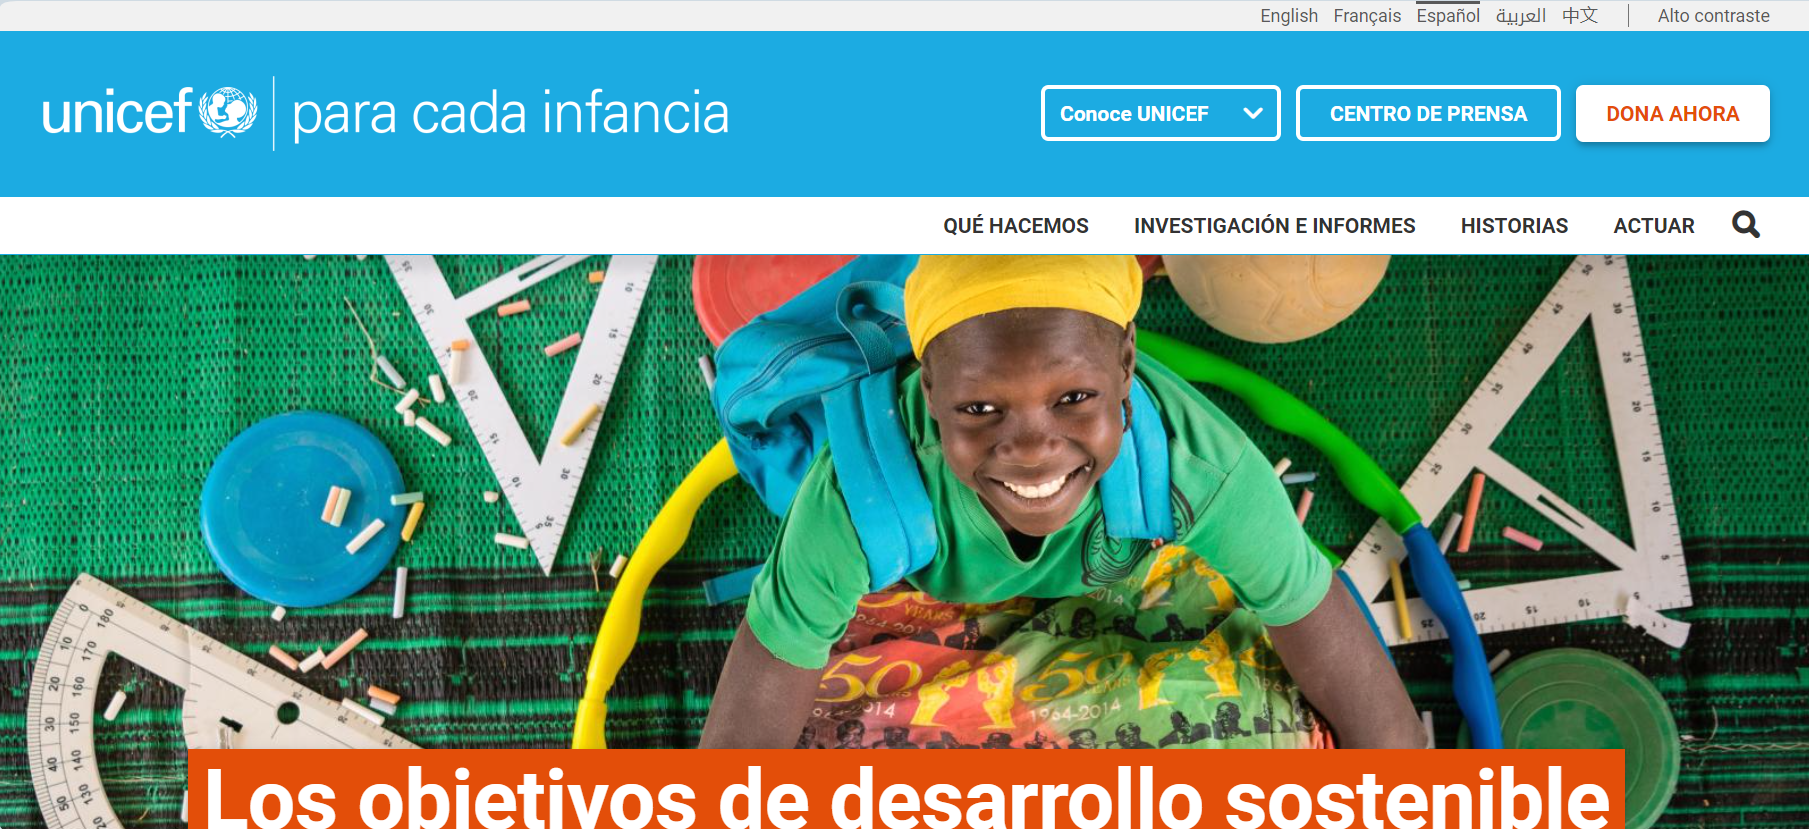
\includegraphics[width=0.9\textwidth, height=10cm, keepaspectratio]{\paginaUnicef}}
        \vspace{0.2cm}\par\textbf{Imagen 3: Captura de la \MYhref{https://www.unicef.org} Página Oficial de UNICEF}\label{fig:imagen-captura-unicef}
    \end{center}
    
    Por otra parte, como aplicación hemos elegido \textbf{Telegram} como podemos ver en la \textbf{\hyperref[fig:imagen-captura-telegram]{Imagen 4}} que consiste en una APP de mensajería. Por lo tanto, consideramos que está aplicación es apta para analizar la accesibilidad, ya que \textbf{cualquier persona debe de tener posibilidad de utilizar una aplicación de mensajería}.
    
    \begin{center}
        \efboxsetup{linecolor=black,linewidth=0.5pt}
        \efbox{\includegraphics[width=\textwidth, height=10cm, keepaspectratio]{\aplicacionTelegram}}\vspace{0.2cm}\par
        \textbf{Imagen 4: Captura de Telegram\label{fig:imagen-captura-telegram}}
    \end{center}
                    
    Para llevar a cabo esta evaluación, hemos utilizado la herramienta de evaluación de accesibilidad web \MYhref{https://wave.webaim.org/}{"\textbf{WebAIM WAVE}"}, junto con las métricas establecidas y consolidado por el \MYhref{https://www.w3.org/WAI/}{\textit{Consorcio World Wide Web (\textbf{W3})}} en sus \MYhref{https://www.w3.org/WAI/standards-guidelines/wcag/}{ \textit{Pautas de Accesibilidad al Contenido Web (\textbf{WCAG})}}. Esto nos permite evaluar tanto aspectos técnicos como la usabilidad y la experiencia general del usuario en el sitio web de \textbf{UNICEF} y \textbf{Telegram}.

    %%%%%%%%%%%%%%%%%%%%%%%%%%%%%%%%%%%%%%%%%%%%%%%%%%%
    % Evaluacion del sitio web de UNICEF
    %%%%%%%%%%%%%%%%%%%%%%%%%%%%%%%%%%%%%%%%%%%%%%%%%%%
    \subsection{Evaluación de accesibilidad web de UNICEF}
    \subsubsection{Puntos Positivos}
    
    \begin{itemize}
        \item \textbf{Textos Alternativos (Nivel A - Criterio 1.1.1 Contenido de imágenes con texto):} Se proporcionan textos alternativos para las imágenes, cumpliendo con los estándares de accesibilidad.
    
        \item \textbf{Identificación del Idioma de la Página (Nivel AA - Criterio 3.1.2 Idioma de las partes):} Se ha identificado correctamente el idioma de la página, garantizando una experiencia de lectura en español sin acentos innecesarios de otros idiomas.
    \end{itemize}
    
    \subsubsection{Puntos Negativos}
    
    \begin{itemize}
        \item \textbf{Zonas con Poco Contraste (Nivel AA - Criterio 1.4.3 Contraste Mínimo):} Se detectan áreas en la página con bajo contraste como podemos ver en la \textbf{\hyperref[fig:imagen-analsis-unicef]{Imagen 5}}, lo que puede dificultar la lectura para algunas personas.

        \item \textbf{Logo Principal Sin Texto (Nivel A - Criterio 1.1.1 Contenido sin Texto):} El logo principal carece de texto descriptivo, lo que puede dificultar la comprensión para usuarios con discapacidades visuales.

        \item \textbf{La página presenta cambios de color bruscos en algunas secciones}, lo que podría ser perjudicial para personas con epilepsia u otros problemas visuales.
        
        \item Aunque se ofrece \textbf{la opción de cambiar el idioma de la página}, esta función \textbf{no es muy perceptible para el usuario}.
    \end{itemize}
    
    \begin{center}
        \efboxsetup{linecolor=black,linewidth=0.5pt}
        \efbox{\includegraphics[width=\textwidth, height=10cm, keepaspectratio]{\erroresUnicef}}\vspace{0.2cm}\par
        \textbf{Imagen 5: Analisis UNICEF\label{fig:imagen-analsis-unicef}}
    \end{center}
    
    \begin{itemize}
        \item Se detectarón numerosos errores de contraste (59 errores) en la página.
        \item Se encontraron 12 imágenes sin texto alternativo, lo que afecta a la accesibilidad de los usuarios con discapacidades visuales.
        \item Se generaron 42 alertas por texto redundante en la página.
    \end{itemize}


    %%%%%%%%%%%%%%%%%%%%%%%%%%%%%%%%%%%%%%%%%%%%%%%%%%%
    % Evaluacion del sitio web de UNICEF con herramienta
    %%%%%%%%%%%%%%%%%%%%%%%%%%%%%%%%%%%%%%%%%%%%%%%%%%%
    \subsubsection{Evaluación de UNICEF con herramienta}
    
    \begin{itemize}
    	\item \textbf{Elementos Estructurales (Nivel A - Criterio 1.3.1 Información y relaciones):} La página utiliza elementos estructurales de HTML5 de manera efectiva, mejorando la organización de la información.
    			
    	\item \textbf{Textos Alternativos (Nivel A - Criterio 1.1.1 Contenido de imágenes con texto):} Se proporcionan textos alternativos para las imágenes, cumpliendo con los estándares de accesibilidad.
    						
    	\item \textbf{Utilización de ARIA (Nivel A - Criterio 4.1.2 Nombres, roles y valores):} La página hace un buen uso de ARIA para mejorar la accesibilidad.
    
    	\item \textbf{El Responsive Web Design (RWD)} como podemos ver en la \textbf{\hyperref[fig:imagen-rwd-unicef]{Imagen 6}} \textbf{no es óptimo}, ya que se observan \textbf{problemas como desplazamiento lateral en dispositivos moviles} o la \textbf{falta de adaptación de iconos y texto} a diferentes tamaños de pantalla.
    \end{itemize}
    
   \begin{center}
        \efboxsetup{linecolor=black,linewidth=0.5pt}
        \efbox{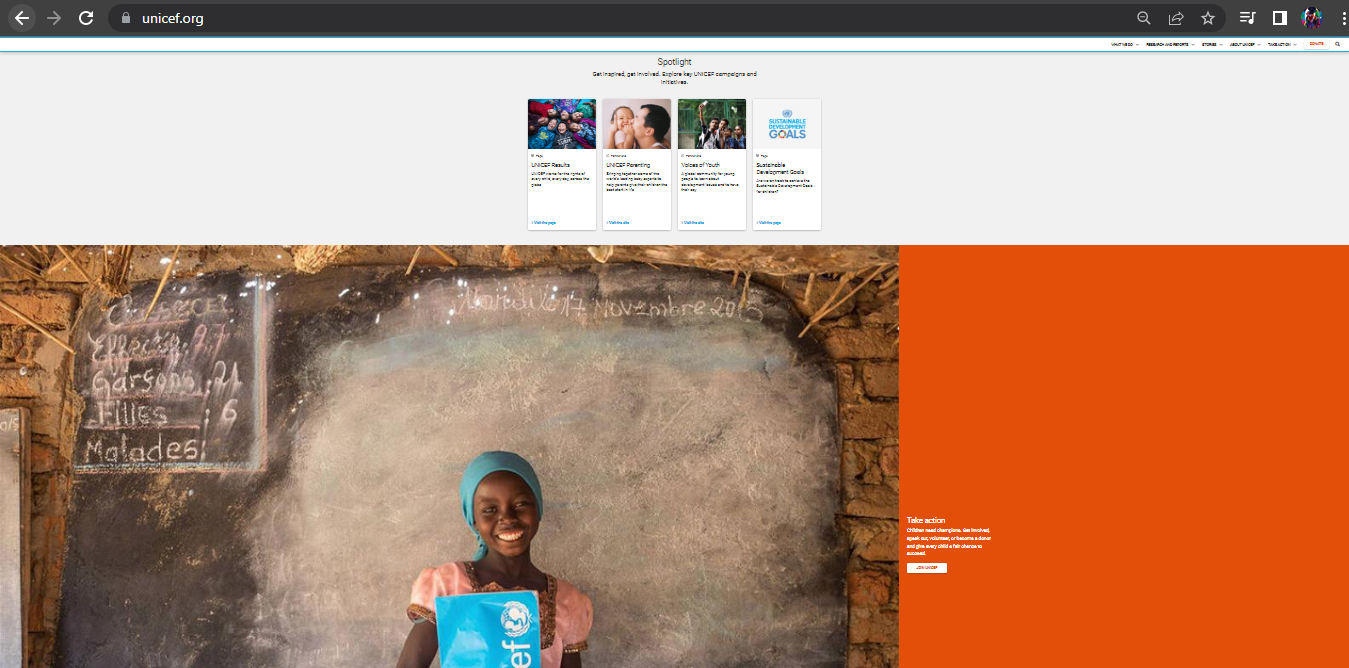
\includegraphics[width=0.9\textwidth, height=10cm, keepaspectratio]{\responsiveUnicef}}\vspace{0.2cm}\par
        \textbf{Imagen 6: Analisis RWD UNICEF\label{fig:imagen-rwd-unicef}}
    \end{center}

    %%%%%%%%%%%%%%%%%%%%%%%%%%%%%%%%%%%%%%%%%%%%%%%%%%%
    % Resumen de la evaluacion
    %%%%%%%%%%%%%%%%%%%%%%%%%%%%%%%%%%%%%%%%%%%%%%%%%%%
    \subsubsection{Resumen de la evaluación\texorpdfstring{\vspace{0.2cm}}{}} 

    
    La herramienta de evaluación de accesibilidad identificó varias áreas de mejora en el sitio web analizado.\vspace{0.2cm}
        
    En particular, problemas de \textbf{diseño responsive} que pueden \textbf{excluir a un gran número de usuarios}. Aunque la navegación se puede realizar con la tecla 'Tab' en toda la página, no es intuitivo para cualquier usuario, además hay partes de la página que puedes llegar, pero si le das a la tecla 'enter' \textbf{no te redirecciona}, con lo cual te vez obligado a utilizar el ratón. La \textbf{ARIA} te indica muchas caracteristicas de los distintos elementos que estructura de la página. \vspace{0.2cm}
    
    En la \textbf{\hyperref[fig:imagen-compromiso-unicef]{Imagen 7}}, podemos apreciar claramente \textbf{la fuerte dedicación de UNICEF a la accesibilidad}. La organización ha creado una \textbf{página específica destinada a la accesibilidad} y está lista para ayudar a cualquier usuario que pueda enfrentar dificultades de accesibilidad en cualquier momento, \textbf{con el objetivo de resolver sus problemas de manera efectiva y rápida}.

    \vspace{5cm}
    \begin{center}
        \efboxsetup{linecolor=black,linewidth=0.5pt}
        \efbox{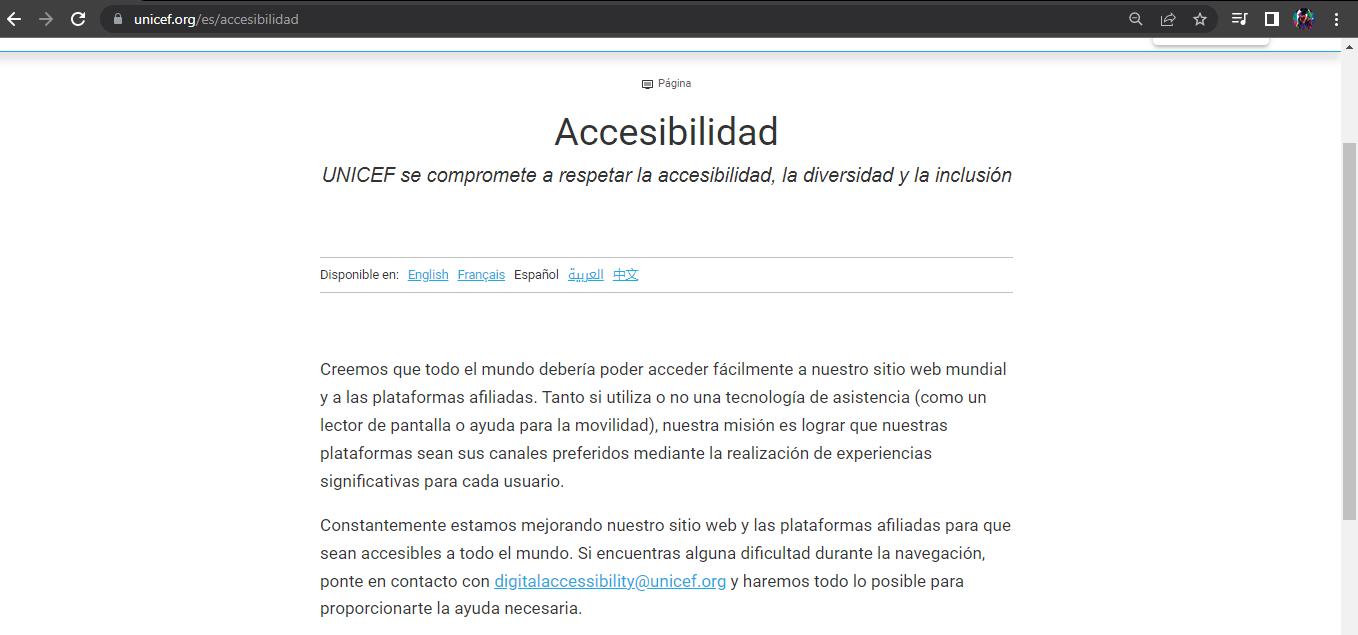
\includegraphics[width=0.9\textwidth, height=10cm, keepaspectratio]{\accesibilidadUnicef}}\vspace{0.2cm}\par
        \textbf{Imagen 7: Compromiso de accesibilidad de UNICEF\label{fig:imagen-compromiso-unicef}}
    \end{center}

    %%%%%%%%%%%%%%%%%%%%%%%%%%%%%%%%%%%%%%%%%%%%%%%%%
    % Evaluacion de TELEGRAM movil con pautas W3 WCAG
    %%%%%%%%%%%%%%%%%%%%%%%%%%%%%%%%%%%%%%%%%%%%%%%%%
            
    \subsection{Evaluación inicial de la accesibilidad de Telegram movil}
    
    %%%%%%%%%%%%%%%%%%%%%%%%%%%
    %  FALTA CONTENIDO DE TELEGRAM
    %%%%%%%%%%%%%%%%%%%%%%%%%%%    
    
    \subsubsection{Puntos Positivos}
    
    \begin{itemize}
        \item \textbf{Contraste de color (color y tipografía):} Telegram proporciona un buen contraste de color como podemos ver en la \textbf{\hyperref[fig:imagen-contraste-telegram]{Imagen 8}} entre el texto y el fondo, lo que facilita la legibilidad para usuarios con discapacidad visual o dificultades de visión.

        \begin{center}
            \efboxsetup{linecolor=black,linewidth=0.5pt}
            \efbox{\includegraphics[width=0.8\textwidth, height=10cm, keepaspectratio]{\coloresTelegram}}\vspace{0.2cm}\par
            \textbf{Imagen 8: Contraste Telegram\label{fig:imagen-contraste-telegram}}
        \end{center}\vspace{0.1cm}

        
        \item \textbf{Tamaño adaptable:} La aplicación de Telegram tiene un diseño adaptable que permite a los usuarios ajustar el tamaño del texto como podemos ver en la \textbf{\hyperref[fig:imagen-longitud-letra]{Imagen 9}} y otros elementos según sus necesidades, lo que mejora la accesibilidad.

        \begin{center}
            \efboxsetup{linecolor=black,linewidth=0.5pt}
            \efbox{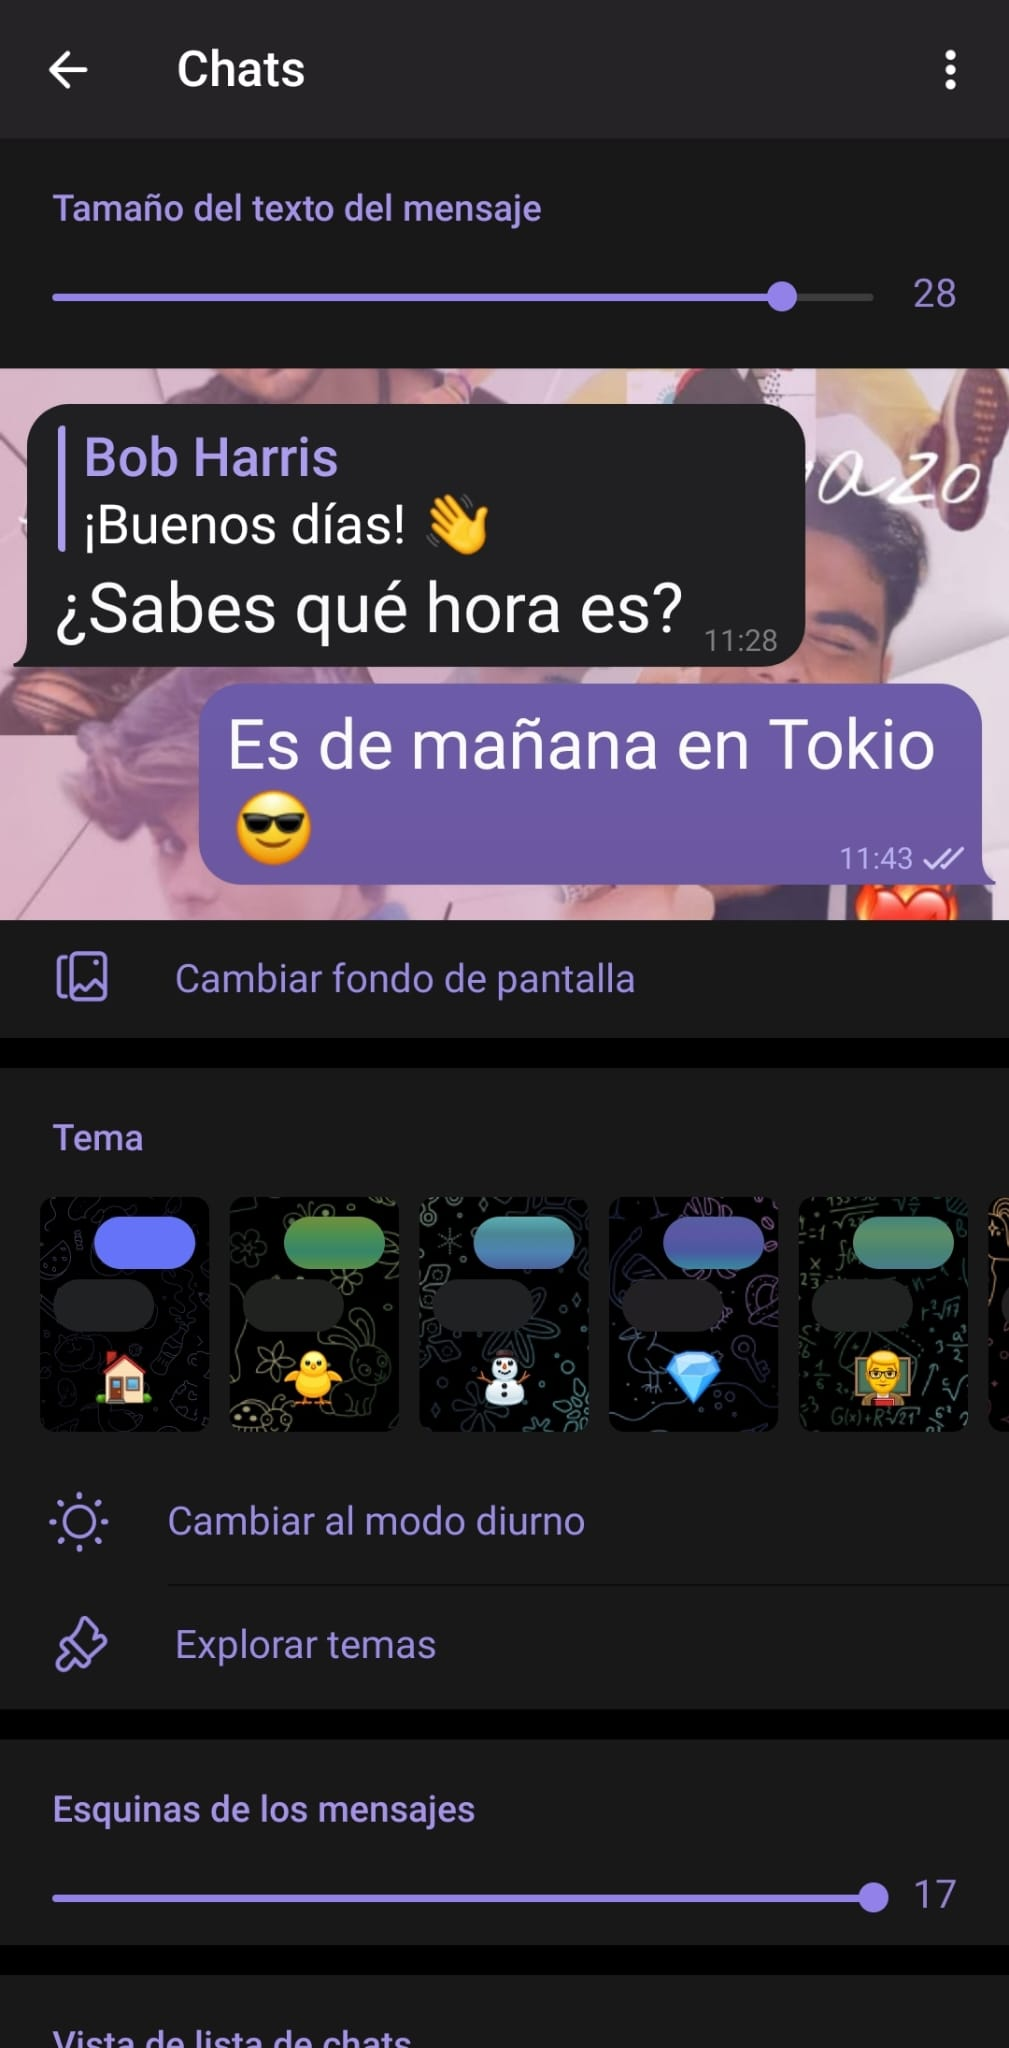
\includegraphics[width=0.8\textwidth, height=10cm, keepaspectratio]{\letraTelegram}}\vspace{0.2cm}\par
            \textbf{Imagen 9: Tamaño de letra\label{fig:imagen-longitud-letra}}
        \end{center}\vspace{0.1cm}
        
        \item \textbf{Facilidad de deshacer:} La función de deshacer en la aplicación permite a los usuarios corregir errores fácilmente, lo que es beneficioso para aquellos con discapacidades cognitivas o destrezas motoras limitadas.
        
        \item \textbf{Información de feedback:} Telegram proporciona información de retroalimentación clara como se puede ver en la \textbf{\hyperref[fig:imagen-telegram-deshacer]{Imagen 10}}, lo que ayuda a los usuarios a comprender las acciones que están realizando y si fueron exitosas o no.

        \begin{center}
            \efboxsetup{linecolor=black,linewidth=0.5pt}
            \efbox{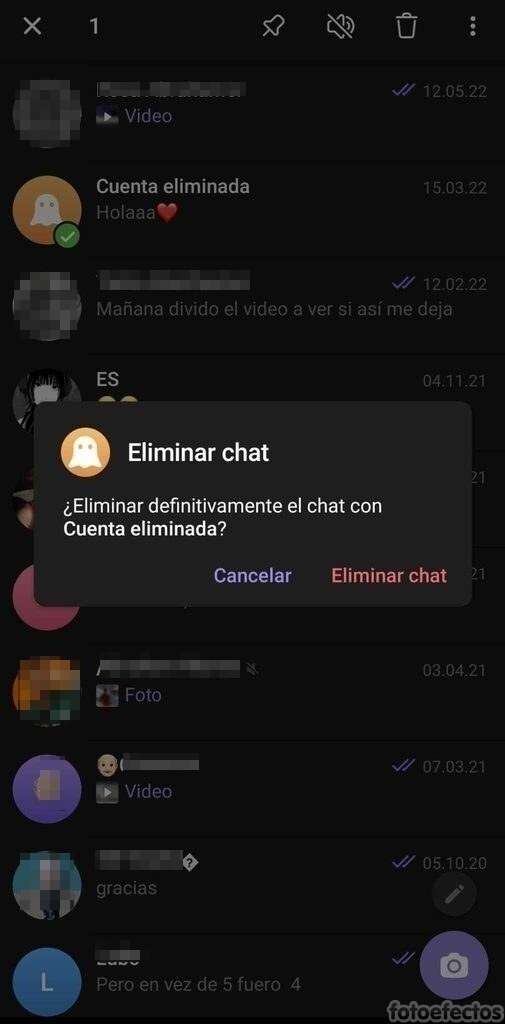
\includegraphics[width=0.8\textwidth, height=10cm, keepaspectratio]{\asegurarTelegram}}\vspace{0.2cm}\par
            \textbf{Imagen 10: POP UP de confirmación\label{fig:imagen-telegram-deshacer}}
        \end{center}\vspace{0.1cm}

        
        \item \textbf{Soporte de lector de pantalla:} La aplicación es compatible con lectores de pantalla, lo que facilita su uso por parte de usuarios con discapacidad visual.
        
        \item \textbf{Navegación sencilla (sin necesidad de clics precisos):} Telegram permite la navegación sencilla, donde los usuarios pueden desplazarse hacia arriba y hacia abajo con gestos táctiles en lugar de requerir clics precisos, lo que facilita la interacción para personas con discapacidades motoras.
        
        \item \textbf{Elección de distintos idiomas:} La disponibilidad de múltiples idiomas en la aplicación de Telegram como se puede ver en la  \textbf{\hyperref[fig:imagen-idioma-telegram]{Imagen 11}} mejora la accesibilidad para usuarios que hablan diferentes lenguajes, lo que es un aspecto positivo para la diversidad cultural y lingüística.

        \begin{center}
            \efboxsetup{linecolor=black,linewidth=0.5pt}
            \efbox{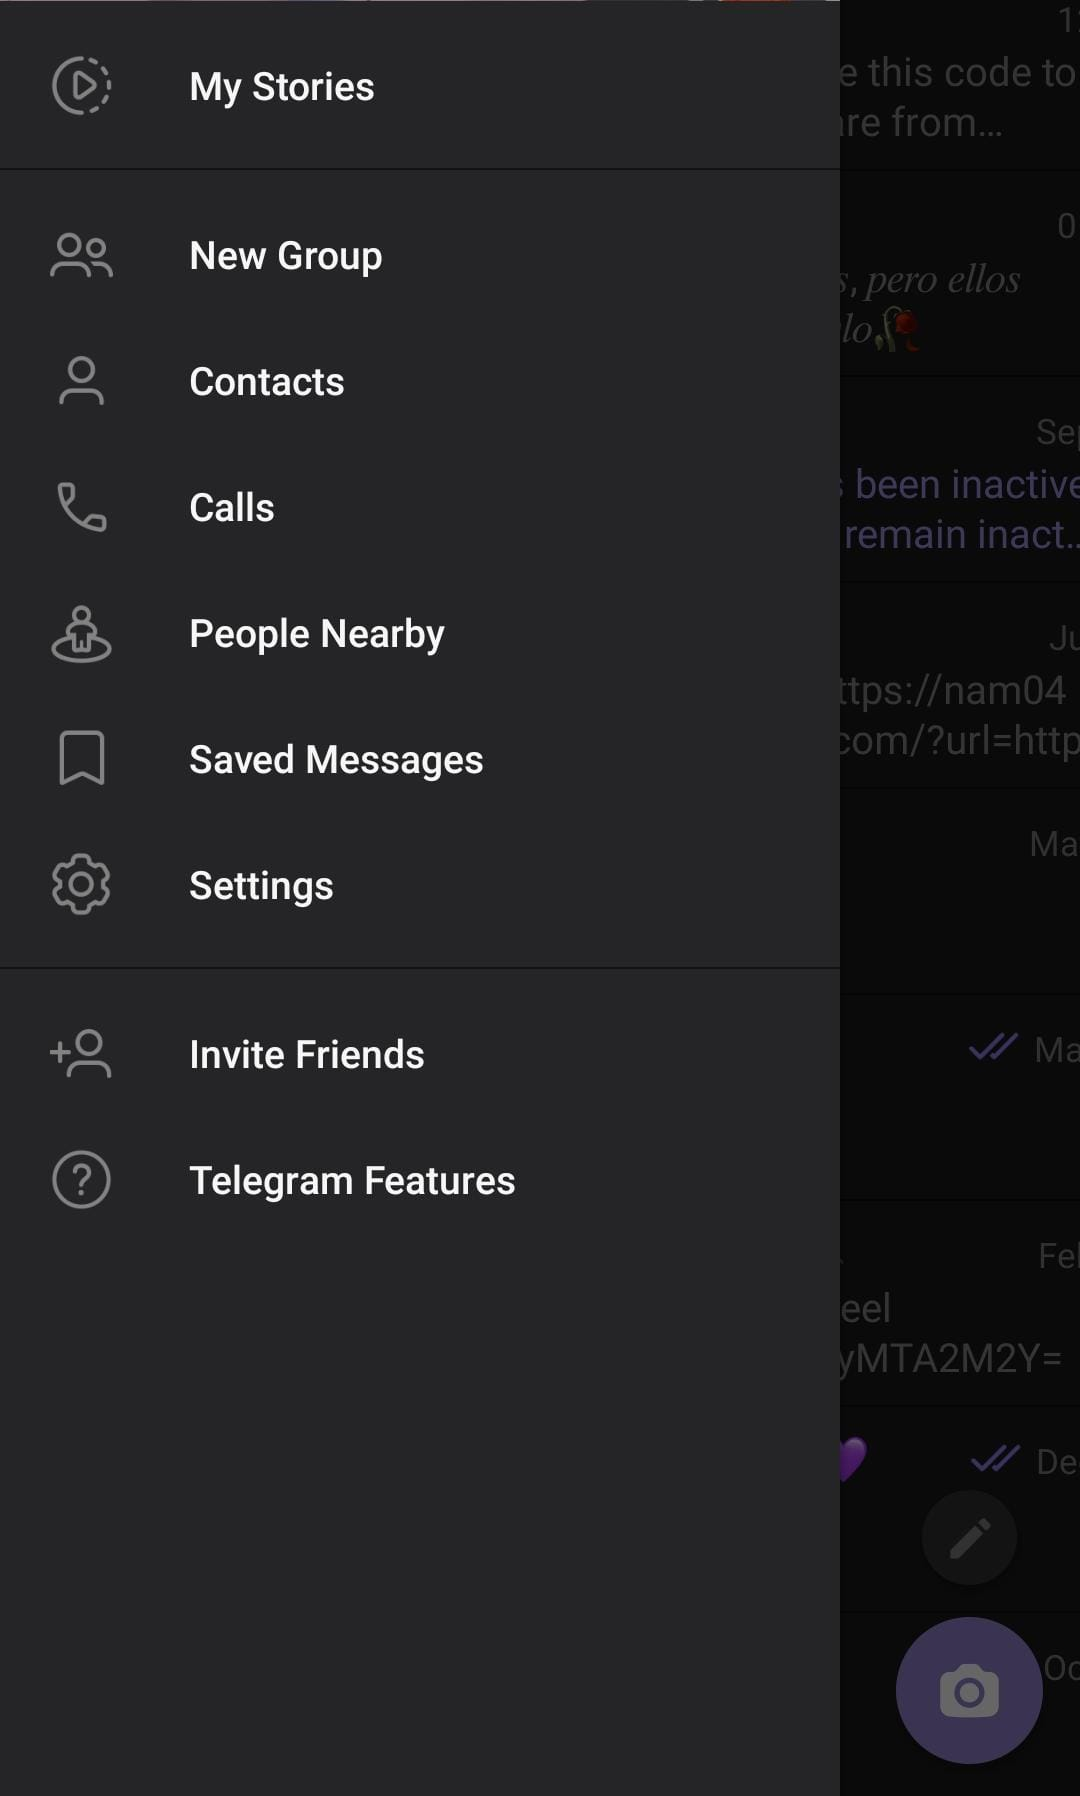
\includegraphics[width=0.8\textwidth, height=10cm, keepaspectratio]{\idiomaTelegram}}\vspace{0.2cm}\par
            \textbf{Imagen 11: Idioma\label{fig:imagen-idioma-telegram}}
        \end{center}\vspace{0.1cm}
    \end{itemize}

    
    \subsubsection{Puntos Negativos}
    \begin{itemize}
        \item \textbf{Videos sin subtítulos (Nivel A - Criterio 1.2.1 Audio-only y Video-only pregrabado:} Este punto significa que los videos en la aplicación móvil de Telegram no proporcionan subtítulos, lo que dificulta la accesibilidad para personas con discapacidad auditiva. Para cumplir con esta pauta, Telegram debería ofrecer la opción de activar subtítulos en sus videos para garantizar que todos los usuarios puedan acceder al contenido.
        
        \item \textbf{Audios sin transcripción (Nivel AA - Criterio 1.2.5 Audio Descriptivo):} Esta desventaja implica que los audios en la aplicación no cuentan con transcripciones, lo que puede dificultar el acceso a personas con discapacidad visual. Para abordar esto, Telegram podría proporcionar transcripciones de audio, lo que permitiría a los usuarios leer el contenido de los audios en lugar de depender únicamente del audio.
        
        \item \textbf{Falta de tiempo de espera en la aplicación (Nivel AAA - Criterio 2.2.6 Timeouts):} Esto sugiere que la aplicación no proporciona suficiente tiempo para que los usuarios completen acciones antes de que expiren las sesiones o las tareas. Para cumplir con esta pauta como se puede ver en la \textbf{\hyperref[fig:imagen-deshacer-telegram-undo]{Imagen 12}}, Telegram podría extender los tiempos de espera o permitir que los usuarios configuren tiempos de espera más largos.
        
        \begin{center}
            \efboxsetup{linecolor=black,linewidth=0.5pt}
            \efbox{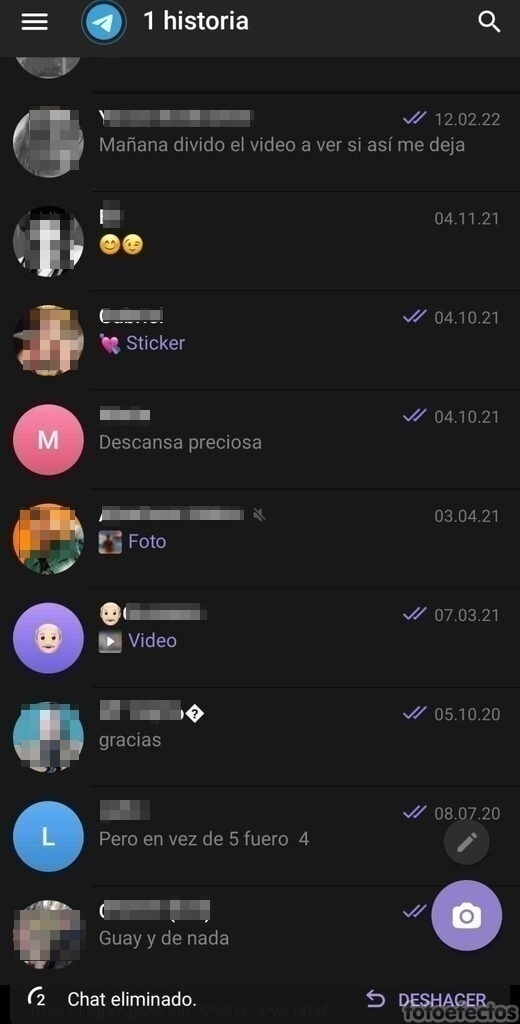
\includegraphics[width=0.8\textwidth, height=10cm, keepaspectratio]{\deshacerTelegram}}\vspace{0.2cm}\par
            \textbf{Imagen 12: Deshacer Telegram\label{fig:imagen-deshacer-telegram-undo}}
        \end{center}\vspace{0.1cm}
        
        \item \textbf{Única forma de autenticación (por mensaje) dependiente de las funciones cognitivas (Nivel AA - Criterio 3.3.8 Autenticación accesible (mínima)):} Esto indica que la aplicación de Telegram solo ofrece autenticación a través de mensajes como podemos ver en la \textbf{\hyperref[fig:imagen-numero-telefono-telegram]{Imagen 13}} y en la \textbf{\hyperref[fig:imagen-mensaje-telefono-telegram]{Imagen 14}}, lo que puede ser un obstáculo para usuarios con limitaciones cognitivas. Para mejorar la accesibilidad, Telegram podría considerar agregar opciones de autenticación adicionales que sean más accesibles para un grupo más amplio de usuarios.
        
        \begin{center}
            \efboxsetup{linecolor=black,linewidth=0.5pt}
            \efbox{\includegraphics[width=0.8\textwidth, height=10cm, keepaspectratio]{\numeroTelefono}}\vspace{0.2cm}\par
            \textbf{Imagen 13: Número de Teléfono\label{fig:imagen-numero-telefono-telegram}}
        \end{center}\vspace{0.1cm}
        
        \begin{center}
            \efboxsetup{linecolor=black,linewidth=0.5pt}
            \efbox{\includegraphics[width=0.8\textwidth, height=10cm, keepaspectratio]{\mensajeTelefono}}\vspace{0.2cm}\par
            \textbf{Imagen 14: Mensaje Teléfono\label{fig:imagen-mensaje-telefono-telegram}}
        \end{center}\vspace{0.1cm}
    \end{itemize}    
    
    
    \subsubsection{Resumen de la Evaluación}

    % Contenido de Telegram
    \textbf{Telegram presenta aspectos positivos}, tales como una interfaz adaptable, retroalimentación clara y soporte para lectores de pantalla, que mejoran la accesibilidad de la aplicación. Sin embargo, también se identifican \textbf{áreas de mejora}, como la falta de subtítulos en videos y la dependencia de una única forma de autenticación basada en mensajes. La optimización de estos aspectos es esencial para hacer que la aplicación sea más accesible y beneficiosa para un público más amplio.
    
    %%%%%%%%%%%%%%%%%%%%%%%%%%%
    % Conclusiones de la pagina
    %%%%%%%%%%%%%%%%%%%%%%%%%%%
    \section{Conclusiones}
    \label{sec:conclusiones_referencias}

    En el proceso de evaluación de accesibilidad web de la página oficial de \textbf{UNICEF} y la aplicación móvil \textbf{Telegram}, hemos identificado tanto aspectos positivos como áreas de mejora que son esenciales para garantizar la accesibilidad a un público diverso. A continuación, resumimos nuestras conclusiones:
    
    \textbf{Para UNICEF}:
    \begin{itemize}
        \item \textbf{UNICEF ha demostrado un compromiso visible con la accesibilidad web} al crear una página específica destinada a la accesibilidad y proporcionar recursos para ayudar a los usuarios con dificultades de accesibilidad.
        \item Sin embargo, existen áreas de mejora, como la \textbf{falta de contraste} en algunas secciones y la \textbf{falta de texto descriptivo en el logo principal}.
        \item La \textbf{navegación y la experiencia del usuario pueden mejorarse}, especialmente en dispositivos móviles, para garantizar que todos los usuarios puedan acceder y utilizar los recursos de UNICEF de manera efectiva.
    \end{itemize}
    
    \textbf{Para Telegram}:
    \begin{itemize}
        \item Telegram presenta aspectos positivos, como el \textbf{contraste de color, la adaptabilidad del tamaño y el soporte de lectores de pantalla}, que mejoran su accesibilidad.
        \item Sin embargo, existen desventajas importantes, como la \textbf{falta de subtítulos en videos, la ausencia de transcripciones de audio, la falta de tiempo de espera} y la \textbf{dependencia de una única forma de autenticación basada en mensajes}.
        \item Mejorar estas áreas de accesibilidad es esencial para garantizar que Telegram sea accesible para un público más amplio y diverso.
    \end{itemize}

    \newpage
    
    En resumen, tanto \textbf{UNICEF} como \textbf{Telegram} pueden mejorar su accesibilidad al abordar las áreas identificadas en esta evaluación. Esto no solo cumple con las pautas y estándares de accesibilidad web, sino que también contribuye a crear un entorno en línea más inclusivo y accesible para todos.
    
    %%%%%%%%%%%%%%%%%%%%%%%%%%%
    % Bibliografia de la pagina
    %%%%%%%%%%%%%%%%%%%%%%%%%%%
    \addcontentsline{toc}{section}{4\hspace{0.4cm}Bibliografía}
    \renewcommand{\refname}{4.\hspace{0.6cm}Bibliografía}
    
    \begin{thebibliography}{9}
        \bibitem{unicef} UNICEF. (Sitio web oficial). Recuperado de \url{https://www.unicef.org}
        
        \bibitem{wave} WAVE Web Accessibility Evaluation Tool. Recuperado de \url{https://wave.webaim.org/}
    
        \bibitem{wcag} W3 WCAG. (Web Content Accessibility Guidelines). Recuperado de \url{https://www.w3.org/TR/WCAG22}
    \end{thebibliography}
\end{document}